% This is samplepaper.tex, a sample chapter demonstrating the
% LLNCS macro package for Springer Computer Science proceedings;
% Version 2.21 of 2022/01/12
%
\documentclass[runningheads]{llncs}
%
\usepackage[T1]{fontenc}
% T1 fonts will be used to generate the final print and online PDFs,
% so please use T1 fonts in your manuscript whenever possible.
% Other font encondings may result in incorrect characters.
%
\usepackage{graphicx}
% Used for displaying a sample figure. If possible, figure files should
% be included in EPS format.
%
% If you use the hyperref package, please uncomment the following two lines
% to display URLs in blue roman font according to Springer's eBook style:
%\usepackage{color}
%\renewcommand\UrlFont{\color{blue}\rmfamily}
%\urlstyle{rm}
%

%\usepackage[utf8]{inputenc} % кодировка
\usepackage[english]{babel} % Русские и английские переносы
\usepackage{cite}              % для корректного оформления литературы
\usepackage{enumitem}
\usepackage{amsmath} 


\begin{document}
%
\title{Parallel global optimization algorithm employing decision trees for launching local methods}
%
\titlerunning{Parallel global optimization algorithm employing decision trees}
% If the paper title is too long for the running head, you can set
% an abbreviated paper title here
%
\author{Konstantin Barkalov\orcidID{0000-0001-5273-2471} \and
Ilya Lebedev\orcidID{0000-0002-8736-0652} \and
Dmitry Silenko\orcidID{0000-0002-2578-9699} }
%
\authorrunning{K. Barkalov et al.}
% First names are abbreviated in the running head.
% If there are more than two authors, 'et al.' is used.
%
\institute{Lobachevsky State University of Nizhni Novgorod, Nizhni Novgorod, Russia}
%
\maketitle              % typeset the header of the contribution
%
\begin{abstract}
%В данной работе разработан подход к параллельному запуску локальных методов при решении задачи глобальной оптимизации с помощью алгоритма глобального поиска. Целевая функция задачи задана как черный ящик; предполагается, что она удовлетворяет условию Липшица с априори неизвестной константой. В работе рассматривается метод выбора окрестности локальных экстремумов целевой функции на основе анализа накопленной поисковой информации. Проведение такого анализа с использованием методов машинного обучения позволяет принять решение о параллельном запуске локальных методов, что позволяет ускорить сходимость алгоритма. Это предположение было подтверждено результатами численных экспериментов, демонстрирующих ускорение при решении серии тестовых задач.

This paper presents an approach for the parallel launch of local optimization methods within a global search algorithm framework, aimed at solving global optimization problems. The objective function is treated as a black-box and is assumed that it satisfies the Lipschitz condition with an unknown constant. The proposed method focuses on selecting the region of attraction of local extrema of the objective function based on the analysis of accumulated search data. Employing machine learning techniques for this analysis enables informed decisions regarding the parallel execution of local methods, leading to improved algorithm convergence. The effectiveness of this approach is validated through numerical experiments, which demonstrate accelerated performance on a set of benchmark problems.


\keywords{
Global optimization $\cdot$
Multi-extremal functions $\cdot$
Parallel computing $\cdot$
Machine learning $\cdot$
Decision tree $\cdot$}
\end{abstract}
%
%
%



\section{Introduction}

%В настоящей работе рассматриваются параллельные алгоритмы решения многомерных задач глобальной оптимизации. Такие задачи часто возникают в тех случаях, когда необходимо подобрать значения параметров исследуемой математической модели, при которых результаты моделирования лучше всего соответствуют экспериментальным данным. Для решения задач этого класса известно множество алгоритмов: от метаэвристических, основанных на идее случайного поиска \cite{Ferreiro2013,Garcia2014,Langdon2011}, до детерминированных алгоритмов, гарантирующих сходимость к глобальному минимуму \cite{Evtushenko2009,He2008,Paulavicius2011}.
This paper investigates parallel algorithms for solving multidimensional global optimization problems These problems commonly occur when optimizing the parameters of a mathematical model to achieve the best possible agreement between simulation results and experimental observations. Numerous algorithms have been developed to address this class of problems, varying from metaheuristic techniques based on the idea of random search \cite{Ferreiro2013,Garcia2014,Langdon2011} to deterministic algorithms designed to guarantee convergence to a global minimum \cite{Evtushenko2009,He2008,Paulavicius2011}.


%Поскольку в реальных задачах глобальной оптимизации каждое вычисление значения функции (далее \textit{trial}) является операцией, требующей больших вычислительных затрат, количество таких попыток приходится сокращать. Это может быть достигнуто за счет преднамеренного выбора вариантов в ходе поиска оптимального решения, отсекая бесперспективные поисковые под области и исследуя только те, в которых можно найти решение задачи. Алгоритм глобального поиска (АГП) основан на этой идее \cite{Strongin2000}. В настоящей работе мы попытались объединить АГП и метод локальной оптимизации \cite{Nocedal, Kelley}  (метод поиска по образцу Хука-Дживса \cite{HookJeeves}), чтобы уменьшить количество выполняемых испытаний. Решение о запуске локального метода будет приниматься с использованием дерева решений.
In real-world global optimization problems, each function evaluation (hereafter referred to as a \textit{trial}) is a computationally expensive operation, making it necessary to reduce the number of such trials. This may be achieved by the purposeful selection of alternatives during the course of optimization, rejecting unpromising search sub-regions and exploring only those where a solution can be found. The Global Search Algorithm (GSA) is based on this idea \cite{Strongin2000}. In this work, we attempted to combine the GSA and a local optimization method (the Hooke-Jeeves pattern search method \cite{Nocedal, Kelley}) to reduce the number of trials performed. The decision to run the local method will be made using a decision tree.


%%%%%%%%%%%%%%%%%%%%%%%%%%%%%%%%%%%%%%%%%%%%%%%%%%%%%%%%%%%%%%%%%%%%%%%%%%%%%%%%%%%%%%%%%
%%%%%%%%%%%%%%%%%%%%%%%%%%%%%%%%%%%%%%%%%%%%%%%%%%%%%%%%%%%%%%%%%%%%%%%%%%%%%%%%%%%%%%%%%
%%%%%%%%%%%%%%%%%%%%%%%%%%%%%%%%%%%%%%%%%%%%%%%%%%%%%%%%%%%%%%%%%%%%%%%%%%%%%%%%%%%%%%%%%


%Классические алгоритмы локальной оптимизации предназначены для нахождения единственного экстремума (локального минимума или максимума) в окрестности начального приближения. В зависимости от используемой информации о целевой функции, эти методы принято классифицировать на:

Classical local optimization algorithms are designed to find a single extremum (local minimum or maximum) in the neighborhood of an initial guess. Depending on the information used about the objective function, these methods are typically classified as:
\begin{itemize}
	\item Zero-order methods, which use only function values;
	\item First-order methods (gradient methods), requiring the computation of first derivatives;
	\item Second-order methods (e.g., Newton's method), which require the computation of the matrix of second derivatives (Hessian).
\end{itemize}


%Важно подчеркнуть, что применение градиентных методов (первого и, в особенности, второго порядка) для оптимизации функций типа черного ящика сопряжено с фундаментальными трудностями. Основная проблема заключается в отсутствии аналитического описания функции, что делает невозможным прямое вычисление производных и приводит к необходимости их численной оценки, что, в свою очередь, может быть вычислительно затратно и вносить дополнительные погрешности \cite{Kelley}. В связи с этим, в рамках данного исследования дальнейшее рассмотрение будет ограничено исключительно методами нулевого порядка, не требующими вычисления производных.
It is important to emphasize that the application of gradient methods (first-order and, especially, second-order) to the optimization of black-box functions is associated with fundamental difficulties. The main problem lies in the absence of an analytical description of the function, which makes direct computation of derivatives impossible and leads to the need for their numerical estimation. This, in turn, can be computationally expensive and introduce additional errors \cite{Kelley}. In light of this, the remainder of this study will be limited exclusively to zero-order methods, which do not require the computation of derivatives.


%Ключевой вопрос при гибридизации глобального и локального поиска заключается в определении оптимального момента для запуска локального метода. Для решения этой задачи предлагается использовать адаптивный алгоритм, основанный на машином обучении, а именно на построении дерева решений.
%На первоначальном этапе глобального поиска информация о поведении целевой функции накапливается в виде набора вычисленных значений в точках испытаний. Эти данные используются для обучения модели дерева решений. Обученная модель строит кусочно-постоянную аппроксимацию целевой функции, которая позволяет прогнозировать её поведение в ещё не исследованных областях.
%Механизм принятия решения о запуске локального поиска заключается в следующем: для точки, подозрительной на наличие в её окрестности локального минимума, с помощью аппроксимирующей модели анализируются значения в соседних точках. На основе этого анализа делается вывод о том, попадает ли следующая точка испытания глобального алгоритма в область притяжения данного локального минимума. Это позволяет своевременно запустить локальную оптимизацию для эффективного уточнения решения в данной области.

A key question when hybridizing global and local search is determining the optimal moment to initiate the local method. To address this, we propose using an adaptive algorithm based on machine learning, specifically on building a decision tree.

In the initial phase of the global search, information about the behavior of the objective function is accumulated in the form of a set of computed values at trial points. This data is used to train a decision tree model. The trained model constructs a piecewise-constant approximation of the objective function, which allows predicting its behavior in unexplored regions.

The mechanism for deciding when to initiate local search is as follows: for a point suspected of having a local minimum in its vicinity, the approximating model is used to analyze values in neighboring points. Based on this analysis, a conclusion is drawn as to whether the next trial point of the global algorithm falls within the basin of attraction of this local minimum. This allows timely initiation of local optimization for effective refinement of the solution in that region.

The content of this paper is structured in the following manner. 
Section \ref{SecA} addresses the methodological basis of the research. It outlines the main idea of the global search algorithm used and details the computational rules of its operation. Furthermore, the section includes a description of the employed local optimization method (zero-order) and justifies the technique for constructing a function approximation using decision trees.
Section \ref{SecGSA} presents the key contribution of this work: a novel hybrid algorithm integrating global search with local refinement, managed via predictions from a decision tree model.
Section \ref{SecR} contains the results of computational experiments conducted on a parallel computing system, their analysis and interpretation, and the formulation of the main concluding remarks.

%%%%%%%%%%%%%%%%%%%%%%%%%%%%%%%%%%%%%%%%%%%%%%%%%%%%%%%%%%%%%%%%%%%%%%%%%%%%%%%%%%%%%%%%%
%%%%%%%%%%%%%%%%%%%%%%%%%%%%%%%%%%%%%%%%%%%%%%%%%%%%%%%%%%%%%%%%%%%%%%%%%%%%%%%%%%%%%%%%%
%%%%%%%%%%%%%%%%%%%%%%%%%%%%%%%%%%%%%%%%%%%%%%%%%%%%%%%%%%%%%%%%%%%%%%%%%%%%%%%%%%%%%%%%%

\section{Problem statement and solution strategies}\label{SecA}

We consider the problem of finding the global minimum of the function $\varphi(y)$ over a hyperinterval $D$, 
\begin{equation} \label{sec:problem}   
	\varphi(y^*) = min\{\varphi(y):y\in D\}, D = \{y \in R^N : a_i \leq y_i \leq b_i, 1 \leq i \leq N \},
\end{equation}
where $a,b \in R$ are given vectors.

We assume that the function satisfies the Lipschitz condition 
\begin{displaymath} 
	|\varphi(y_1)-\varphi(y_2)|\leq L\parallel y_1-y_2 \parallel ,y_1,y_2 \in D, 0<L< \infty, 
\end{displaymath}
with an a priori unknown constant $L$, which corresponds to a bounded change in the function's values for a bounded change in the argument.
This assumption can be viewed (in the context of real-world problems) as reflecting the limited power generating changes in the simulated system.

The numerical solution of the problem (\ref{sec:problem}) reduces to constructing an estimate $y_k^\ast\in D$ that corresponds to some notion of proximity to a point $y^\ast$ (e.g., ${ ||y^\ast-y}_k^\ast||\le\ \varepsilon$, where $\varepsilon\geq0$ is a given accuracy) based on a finite number $k$ of computed values of the objective function. With respect to the class of problems considered, we assume that the objective function $\varphi(y)$ can be algorithmically defined through the execution of a subroutine.

When solving multidimensional problems, dimensionality reduction is employed (i.e., reducing the multidimensional problem to an equivalent one-dimensional one) using Peano curves. These curves allow transforming the multidimensional optimization problem in the region $D$ into a one-dimensional minimization problem on the interval [0, 1].
\begin{displaymath}
	\varphi(y(x^\ast))\ =\min\{\varphi(y(x)): x\in [0,1]\},
\end{displaymath}
where function $\varphi(y(x^\ast))$ satisfies the more general Hölder condition
\begin{displaymath}
	\left|\varphi (y \left(x_1\right))- \varphi (y \left(x_2\right)\right )|\le\ H\left|x_1-x_2\right|^\frac{1}{N},\ x_1,\ x_2\epsilon[0,1].
\end{displaymath} 

Consequently, rather than addressing the original problem of minimizing the function $\varphi(y)$ within the domain $D$, we can consider minimizing the one-dimensional function $f(x)=\varphi(y(x))$, subject to the Hölder condition for $x \in [0, 1]$.
%%%%%%%%%%%%%%%%%%%%%%%%%%%%%%%%%%%%%%%%%%%%%%%%%%%%%%%%%%%%%%%%%%%%%%%%%%%%%%%%%%%%%%%%%
%%%%%%%%%%%%%%%%%%%%%%%%%%%%%%%%%%%%%%%%%%%%%%%%%%%%%%%%%%%%%%%%%%%%%%%%%%%%%%%%%%%%%%%%%
%%%%%%%%%%%%%%%%%%%%%%%%%%%%%%%%%%%%%%%%%%%%%%%%%%%%%%%%%%%%%%%%%%%%%%%%%%%%%%%%%%%%%%%%%
This approach is discussed in the works \cite{Sergeyev2022, Usova2024}.
%%%%%%%%%%%%%%%%%%%%%%%%%%%%%%%%%%%%%%%%%%%%%%%%%%%%%%%%%%%%%%%%%%%%%%%%%%%%%%%%%%%%%%%%%
%%%%%%%%%%%%%%%%%%%%%%%%%%%%%%%%%%%%%%%%%%%%%%%%%%%%%%%%%%%%%%%%%%%%%%%%%%%%%%%%%%%%%%%%%
%%%%%%%%%%%%%%%%%%%%%%%%%%%%%%%%%%%%%%%%%%%%%%%%%%%%%%%%%%%%%%%%%%%%%%%%%%%%%%%%%%%%%%%%%


%Чтобы определить, в какой момент лучше запускать локальный метод в рамках глобального поиска, воспользуемся алгоритмом, основанным на дереве решений. На первом этапе поиска происходит накопление поисковой информации в виде результатов выполненных испытаний. На основе результатов испытаний проводилось обучение дерева решений, позволяющего получать кусочно-постоянную аппроксимацию целевой функции и на ее основе прогнозировать поведение целевой функции. 
To identify when to best launch a local method  within the framework of a global search, we employ an algorithm based on a decision tree  \cite{Barkalov2023_2}. The first stage of the search involves accumulating search information in the form of results from performed trials. Based on these trial results, a decision tree is trained, allowing us to obtain a piecewise-constant approximation of the objective function and, consequently, to predict the behavior of the objective function.

%Дерево решений — это инструмент для автоматизированного анализа больших массивов данных, применяемый в машинном обучении. Его можно использовать как для решения задач классификации, так и для регрессии. В случае построения регрессии каждому листу дерева присваивается константа. Поэтому полученная аппроксимирующая функция является кусочно-постоянной. В нашем случае дерево решений строит функцию $\psi(y)$ как кусочно-постоянную аппроксимацию $\varphi(y)$ в области поиска. Обозначим значение, вычисленное деревом решений в точке $y$, как $z' = \psi(y)$.
%A decision tree is a tool for automated analysis of large datasets used in machine learning. It can be used for both classification and regression problems. In the case of regression, each leaf of the tree is assigned a constant. Therefore, the resulting approximating function is piecewise-constant. In our case, the decision tree constructs a function $\psi(y)$ as a piecewise-constant approximation of $\varphi(y)$ in the search space. Let $z' = \psi(y)$ denote the value computed by the decision tree at point $y$.



%%%%%%%%%%%%%%%%%%%%%%%%%%%%%%%%%%%%%%%%%%%%%%%%%%%%%%%%%%%%%%%%%%%%%%%%%%%%%%%%%%%%%%%%%
%%%%%%%%%%%%%%%%%%%%%%%%%%%%%%%%%%%%%%%%%%%%%%%%%%%%%%%%%%%%%%%%%%%%%%%%%%%%%%%%%%%%%%%%%
%%%%%%%%%%%%%%%%%%%%%%%%%%%%%%%%%%%%%%%%%%%%%%%%%%%%%%%%%%%%%%%%%%%%%%%%%%%%%%%%%%%%%%%%%

%Дерево решений представляет собой широко распространенный и мощный инструмент машинного обучения, предназначенный для автоматического выявления сложных зависимостей в больших многомерных массивах данных. В контексте нашего исследования данный метод применяется для построения вспомогательной аппроксимирующей модели с целью ускорения процесса глобальной оптимизации.

%С формальной точки зрения, используемая модель представляет собой бинарное дерево, то есть такую древовидную структуру, где каждый внутренний (нелистовой) узел имеет ровно два дочерних узла. Этот универсальный инструмент может применяться для решения двух типов задач: классификации и регрессии. В задачах классификации результатом обработки объекта является отнесение его к одному из классов, для чего каждый терминальный узел (лист) дерева помечается соответствующей меткой класса, при этом несколько листьев могут содержать идентичные метки. В задачах регрессии, что более релевантно для нашего случая, каждому листу ставится в соответствие некоторое постоянное (скалярное) значение. Таким образом, итоговая регрессионная модель представляет собой кусочно-постоянную функцию, принимающую на различных участках области определения фиксированные значения.

%В рамках предложенного подхода дерево решений используется для построения вспомогательной функции $\psi(y)$, которая служит кусочно-постоянной аппроксимацией некоторой заданной функции $\varphi(y)$ в пределах исследуемой области поиска. Значение, вычисляемое данной моделью в произвольной точке $y$, обозначается как $z' = \psi(y)$. Эта аппроксимация позволяет эффективно оценивать поведение целевой функции и принимать решения о дальнейшем направлении вычислительных ресурсов в процессе оптимизации.

A decision tree is a widespread and powerful machine learning tool designed to automatically identify complex dependencies in large multidimensional datasets. In the context of our research, this method is used to build an auxiliary approximating model in order to accelerate the global optimization process.

From a formal point of view, the model used is a binary tree, that is, a tree structure where each internal (non-leaf) node has exactly two child nodes. This versatile tool can be used to solve two types of problems: classification and regression. In classification tasks, the result of processing an object is to assign it to one of the classes, for which each terminal node (leaf) of the tree is marked with the corresponding class label, while several leaves may contain identical labels. In regression problems, which is more relevant for our case, each sheet is assigned a certain constant (scalar) value. Thus, the final regression model is a piecewise constant function that takes fixed values in different parts of the definition area.

In the framework of the proposed approach, a decision tree is used to construct an auxiliary function $\psi(y)$, which serves as a piecewise constant approximation of a given function $\varphi(y)$ within the search area under study. The value calculated by this model at any point $y$ is denoted as $z' = \psi(y)$. This approximation makes it possible to effectively evaluate the behavior of the objective function and make decisions about the further direction of computing resources in the optimization process.

%%%%%%%%%%%%%%%%%%%%%%%%%%%%%%%%%%%%%%%%%%%%%%%%%%%%%%%%%%%%%%%%%%%%%%%%%%%%%%%%%%%%%%%%%
%%%%%%%%%%%%%%%%%%%%%%%%%%%%%%%%%%%%%%%%%%%%%%%%%%%%%%%%%%%%%%%%%%%%%%%%%%%%%%%%%%%%%%%%%
%%%%%%%%%%%%%%%%%%%%%%%%%%%%%%%%%%%%%%%%%%%%%%%%%%%%%%%%%%%%%%%%%%%%%%%%%%%%%%%%%%%%%%%%%




Fig. \ref{fig:fig2} shows the graph of the objective function $\varphi(y)$; Fig. \ref{fig:fig2_2} presents the corresponding approximation $\psi(y)$ constructed using a decision tree.
\begin{figure}
	\begin{center}
		\begin{minipage}[h]{0.7\linewidth}
			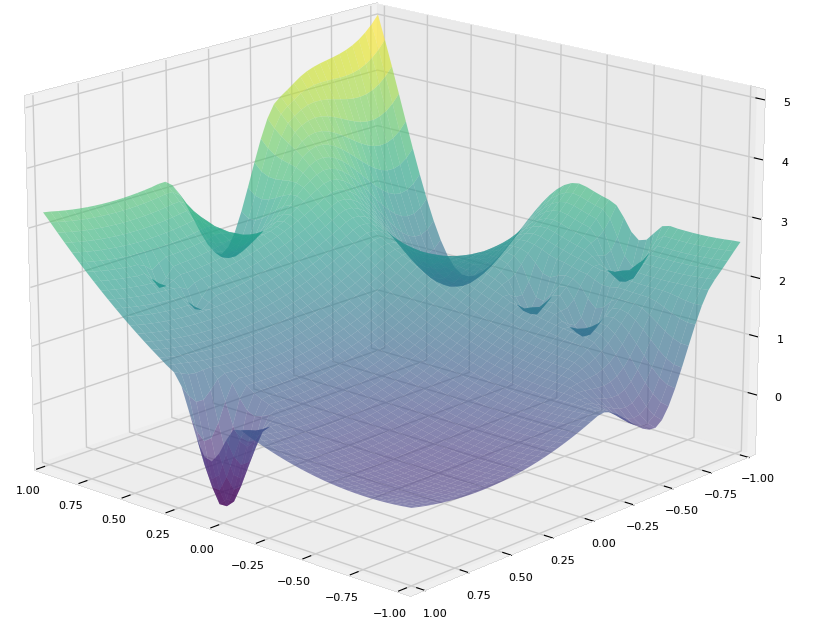
\includegraphics[width=1\linewidth]{figure/fig5.png}
			\caption{Graph of the benchmark objective function $\varphi(y)$} %% подпись к рисунку
			\label{fig:fig2}
		\end{minipage}
	\end{center}
\end{figure}	

\begin{figure}
	\begin{center}
		\begin{minipage}[h]{0.7\linewidth}
			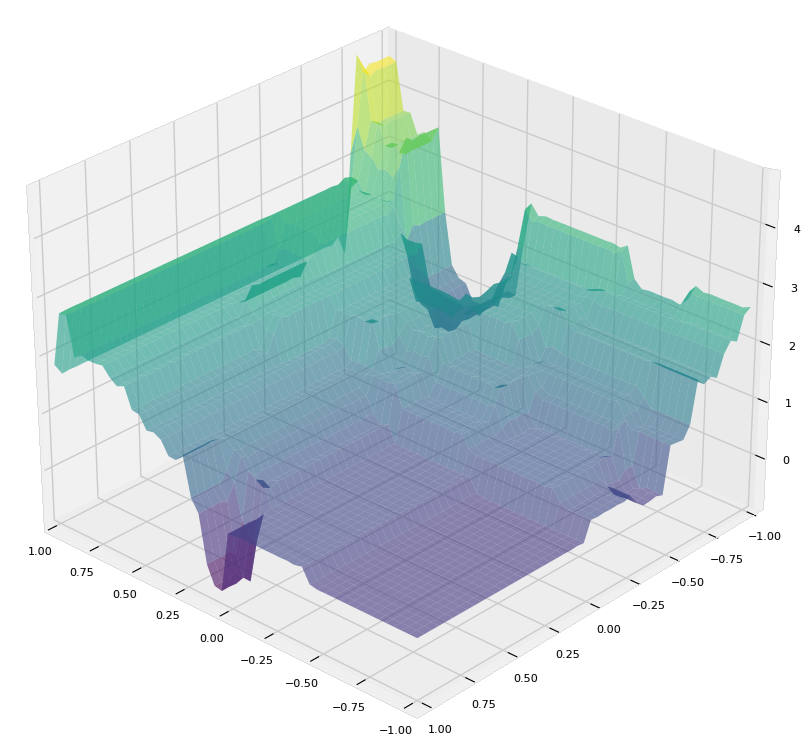
\includegraphics[width=1\linewidth]{figure/fig4.png}
			\caption{Graph of the piecewise-constant approximation $\psi(y)$ of the function $\varphi(y)$} %% подпись к рисунку
			\label{fig:fig2_2}
		\end{minipage}
	\end{center}
\end{figure}	


%При реализации алгоритма поиска областей притяжения локальных минимумов для построения дерева решений использовались алгоритмы из библиотеки OpenCV. OpenCV — это библиотека с открытым исходным кодом алгоритмов компьютерного зрения, обработки изображений и численных алгоритмов общего назначения. Более подробную информацию о дереве решений можно найти в \cite{Brahmbhatt2013}.
To implement the algorithm for identifying the regions of attraction for local minima to construct the decision tree algorithms from the OpenCV library were employed. OpenCV is an open-source library encompassing computer vision algorithms, image processing methods, and general-purpose numerical routines. Detailed information on decision trees may be found in \cite{Brahmbhatt2013}.


%После определения с помощью дерева решений области притяжения локального минимума, из точки ближайшего испытания, проведенного в этой области, запускается локальный метод. Мы использовали метод Хука--Дживса, который относится к классу методов нулевого порядка. Его правила вычисления представляют собой комбинацию исследовательского поиска (для выбора направления) и поиска в выбранном направлении \cite{Himmelblau72}.
Having identified a basin of attraction for a local minimum using the decision tree, a local method is launched from the nearest trial point conducted within that basin. We employed the Hooke-Jeeves method, classified as a zero-order technique. Its computational rules combine an exploratory search (for direction selection) with a search along the selected direction \cite{Himmelblau72}.


%%%%%%%%%%%%%%%%%%%%%%%%%%%%%%%%%%%%%%%%%%%%%%%%%%%%%%%%%%%%%%%%%%%%%%%%%%%%%%%%%%%%%%%%%
%%%%%%%%%%%%%%%%%%%%%%%%%%%%%%%%%%%%%%%%%%%%%%%%%%%%%%%%%%%%%%%%%%%%%%%%%%%%%%%%%%%%%%%%%
%%%%%%%%%%%%%%%%%%%%%%%%%%%%%%%%%%%%%%%%%%%%%%%%%%%%%%%%%%%%%%%%%%%%%%%%%%%%%%%%%%%%%%%%%

The exploratory search is conducted as follows:
\begin{itemize}[label=$\bullet$] 
	\item The step size is determined (it is different for each coordinate direction and can change during the search);
	\item A search step is considered successful if the objective function value at the new point does not exceed the value at the initial point; 
	\item Otherwise, it is necessary to return and take a step in the opposite direction; 
	\item After iterating through all $N$ coordinates, the exploratory search ends; the resulting point is called the base point.
\end{itemize}
The pattern search consists of taking one step from the resulting base point along the line connecting it to the previous base point.


%%%%%%%%%%%%%%%%%%%%%%%%%%%%%%%%%%%%%%%%%%%%%%%%%%%%%%%%%%%%%%%%%%%%%%%%%%%%%%%%%%%%%%%%%
%%%%%%%%%%%%%%%%%%%%%%%%%%%%%%%%%%%%%%%%%%%%%%%%%%%%%%%%%%%%%%%%%%%%%%%%%%%%%%%%%%%%%%%%%
%%%%%%%%%%%%%%%%%%%%%%%%%%%%%%%%%%%%%%%%%%%%%%%%%%%%%%%%%%%%%%%%%%%%%%%%%%%%%%%%%%%%%%%%%

\begin{figure} 
	\begin{center} 
		\begin{minipage}[!h]{1.0\linewidth} 
			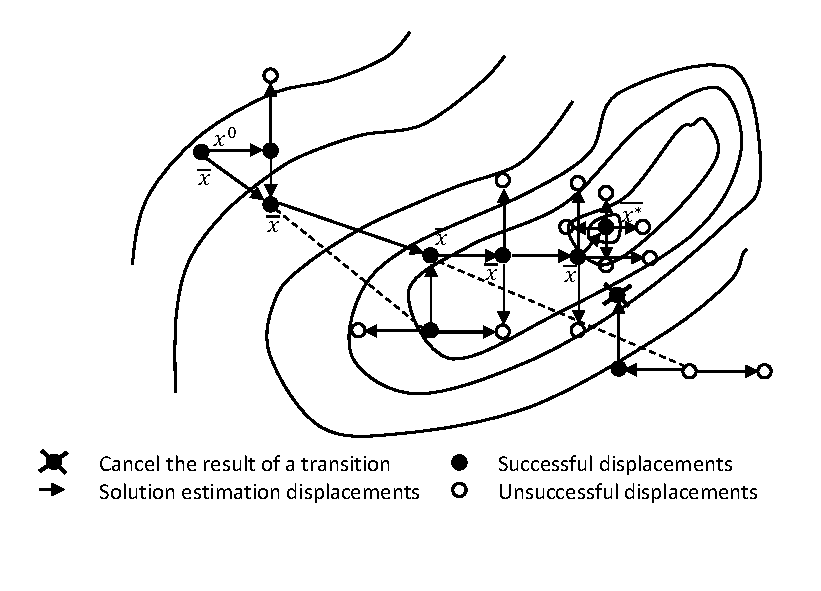
\includegraphics[width=1\linewidth]{figure/fig1.pdf} 
			\caption{An example showing the iterations of the Hooke-Jeeves method} %%  подпись к рисунку 
			\label{fig:fig1} 
		\end{minipage} 
	\end{center} 
\end{figure}	


Fig. \ref{fig:fig1} visually demonstrates the local algorithm in action. Level lines are shown with filled circles representing successful steps and open circles indicating unsuccessful steps from the exploratory search. 


\section{Global search algorithm with local methods starting in parallel}\label{SecGSA}

%TODO
%Здесь нужны общие слова про параллельную программу с несколькими процессами, мастером и рабочими

%%%%%%%%%%%%%%%%%%%%%%%%%%%%%%%%%%%%%%%%%%%%%%%%%%%%%%%%%%%%%%%%%%%%%%%%%%%%%%%%%%%%%%%%%
%%%%%%%%%%%%%%%%%%%%%%%%%%%%%%%%%%%%%%%%%%%%%%%%%%%%%%%%%%%%%%%%%%%%%%%%%%%%%%%%%%%%%%%%%
%%%%%%%%%%%%%%%%%%%%%%%%%%%%%%%%%%%%%%%%%%%%%%%%%%%%%%%%%%%%%%%%%%%%%%%%%%%%%%%%%%%%%%%%%

One way to organize parallel computations on a supercomputer, which has a large number of computational cores and a high thread count per core, is to use synchronous parallel function evaluation.

In the proposed approach, the parallelization scheme follows a ``master-worker'' principle. The master process executes the global search algorithm, accumulates search information, calculates the Lipschitz constant for the objective function based on this information, determines new trial points, and distributes them among the worker processes. The worker processes receive the trial points from the master process, evaluate the function at those points, and send the results back to the master process.

%%%%%%%%%%%%%%%%%%%%%%%%%%%%%%%%%%%%%%%%%%%%%%%%%%%%%%%%%%%%%%%%%%%%%%%%%%%%%%%%%%%%%%%%%
%%%%%%%%%%%%%%%%%%%%%%%%%%%%%%%%%%%%%%%%%%%%%%%%%%%%%%%%%%%%%%%%%%%%%%%%%%%%%%%%%%%%%%%%%
%%%%%%%%%%%%%%%%%%%%%%%%%%%%%%%%%%%%%%%%%%%%%%%%%%%%%%%%%%%%%%%%%%%%%%%%%%%%%%%%%%%%%%%%%


At the initial stage, the master process (let it have the identifier 0) launches $p$ trials in parallel at $p$ different points $\{y\left(x^1\right),y\left(x^2\right),\ldots,y\left(x^p\right)\}$, where preimages $\{x^1,x^2,\ldots,x^p\}$ are form the interval $[0,1]$.
Two preimages are the boundary points $x^1=0, x^p=1$; the remaining preimages are interior points $x^i\in\left(0,1\right),i=2,\ldots,p-1$.

Let us now assume that the algorithm has completed $K \geq 0$ iterations and $k \geq K$ trials have been performed.

%TODO
%Здесь нужно связующее предложение


%%%%%%%%%%%%%%%%%%%%%%%%%%%%%%%%%%%%%%%%%%%%%%%%%%%%%%%%%%%%%%%%%%%%%%%%%%%%%%%%%%%%%%%%%
%%%%%%%%%%%%%%%%%%%%%%%%%%%%%%%%%%%%%%%%%%%%%%%%%%%%%%%%%%%%%%%%%%%%%%%%%%%%%%%%%%%%%%%%%
%%%%%%%%%%%%%%%%%%%%%%%%%%%%%%%%%%%%%%%%%%%%%%%%%%%%%%%%%%%%%%%%%%%%%%%%%%%%%%%%%%%%%%%%%

In each iteration, the algorithm selects several computation points and distributes them to processes in groups. MPI manages this, with process zero handling point distribution and result collection, but remaining computationally idle. Each remaining process receives a group of points, which are computed in parallel using the CPU.

%%%%%%%%%%%%%%%%%%%%%%%%%%%%%%%%%%%%%%%%%%%%%%%%%%%%%%%%%%%%%%%%%%%%%%%%%%%%%%%%%%%%%%%%%
%%%%%%%%%%%%%%%%%%%%%%%%%%%%%%%%%%%%%%%%%%%%%%%%%%%%%%%%%%%%%%%%%%%%%%%%%%%%%%%%%%%%%%%%%
%%%%%%%%%%%%%%%%%%%%%%%%%%%%%%%%%%%%%%%%%%%%%%%%%%%%%%%%%%%%%%%%%%%%%%%%%%%%%%%%%%%%%%%%%


\begin{enumerate}
	
	\item Extract $c = \max(p, |U|)$ trial point coordinates $y^{k+1}=y\left(x^{k+1}\right),...,y^{k+c}=y\left(x^{k+c}\right)$ from the set $U$ (which contains trial point coordinates). If $c < p$, then first perform trials at $n = p - c$ points according to Steps~2--7; otherwise proceed directly to Step~8.
	
	\item Renumber (using subscripts) the points $x^i, 1\leq i\leq k$,  along with the boundary points of the interval $[0, 1]$ in increasing order of their coordinate values
	\begin{equation} 
		\label{agp1_sort} 	0=x_0<\ x_1<\ ...\ <x_{k+1}=1 	
	\end{equation} 
	and associate with them the values $z_i=f(x_i)$. 
	
	\item  Compute the current lower bound $M$ of the unknown Hölder constant $H$: 
	\begin{equation} 
		\label{agp2_mu} 	\mu=max\left\{\frac{|z_i-z_{i-1}|}{{{(x}_i-x_{i-1})}^{1/N}},\ i=1,\ldots,k\right\},\ M=\  \left\{\begin{matrix}r\mu,\ \mu>0,\\1,\ \mu=0,\\\end{matrix}\right.\ 	
	\end{equation} 
	where $r>1$ is the method parameter. This parameter controls the reliability of the algorithm: higher values of $r$ guarantee finding the global minimum, while choosing a smaller value accelerates the convergence of the algorithm.
	
	\item  For each interval $(x_{i-1},x_i), 1\leq i\leq k+1,$ compute a value $R(i)$, called \textit{the characteristic} of the interval, according to the following formulas:
	\begin{equation} 
		\label{agp3_R1} R(1)=2\Delta_1-4\dfrac{z_1}{M}, \; R(k+1)=2\Delta_{k+1}-4\dfrac{z_k}{M}, 
	\end{equation} 
	\begin{equation} 
		\label{agp3_Ri} R(i)=\Delta_i+\dfrac{(z_i-z_{i-1})^2}{M^2\Delta_i}-2\dfrac{z_i+z_{i-1}}{M},1<i<k+1, 
	\end{equation} 
	where \(\Delta_i=(x_i-x_{i-1})^\frac{1}{N}\).
	
	\item   Sort the characteristics  $R\left(i\right),\ 1\leq i \leq k+1,$  in non-increasing order
	\begin{equation} 
		\label{agp4_R_sort} 	R\left(t_1\right)\geq\ R\left(t_2\right)\geq...\geq\ R\left(t_k\right)\geq\ R(t_{k+1}),\  
	\end{equation} 
and select $n$ intervals with indices $t_j, 1 \le j \le n$, that have the largest characteristic values.	
	
	\item Compute the coordinates of the new trial points $y'^{k+j}=y\left(x^{k+j}\right), \ 1\leq j\leq n$, whose preimages are  $x^{k+j}\in\left(x_{t_j-1},x_{t_j}\right)$, according to the following formula:
	\begin{equation}
		\label{agp5_x1}
		x^{k+j}=\frac{x_{t_j}+x_{t_j-1}}{2}-\mathrm{sign}\left(z_{t_j}-z_{t_j-1}\right)\frac{1}{2r}\left[\frac{\left|z_{t_j}-z_{t_j-1}\right|}{M}\right]^N.
	\end{equation}	
	

	
	\item Send to process $j$, $1 \leq j \leq n$, the coordinates of points $y'^{k+1}, \dots, y'^{k+n}$ and notify the process that it needs to perform a single trial.
	
	\item Send to processes $h$, $1 \leq h \leq c$, the coordinates of points $y^{k+1}, \dots, y^{k+c}$ and notify the process that it needs to run a local method.
	
	\item Receive trial results from all $p$ processes and add them to the search information.
	
	\item Add the trial points $y'^{k+1}=y\left(x^{k+1}\right) , \dots, y'^{k+n}=y\left(x^{k+n}\right)$  to the set $V$.
	
	\item If $k < 100N$, go to Step~1.
	
	
	\item Build a decision tree using all the accumulated search information and obtain the approximating function $\psi(y)$.
	
	\item If the decision tree is being used for the first time, construct a uniform grid
	\begin{displaymath} 
		Y'=\{ y'\in R^N:\ a_i\le y'_i \le b_i,\ 1\le i\le N \},
	\end{displaymath} 
	where the number of grid nodes is a parameter of the method.
	
	
	\item Compute the piecewise constant approximation of the function $\psi(y)$ using the decision tree: $Z' = \{ z' = \psi(y'), y' \in Y' \}$.
	
	\item For all points $y' \in V$, find the points $y'_q$ closest to $y'$.
		If no point $y'_q$ has a value smaller than $y'$, add $y'$ to the set $U$.
		Clear the set $V$.
	
	\item Check the stopping criteria.
	
\end{enumerate}

The following $p$ trials are executed in parallel at the points$x^{k+j},\ 1\leq j\leq p$,  computed using formula  (\ref{agp5_x1}). Upon completion of these trials, their results are stored in the search information database, and the algorithm proceeds to compute new trial points. Note that, generally, the trial process in applied optimization problems is far more computationally expensive than computing the coordinates of a point.

The algorithm terminates if the condition \(\Delta_{t_j} < \varepsilon\) is satisfied for at least one value of $t_j,\ 1\le\ j\le\ p$, from (\ref{agp4_R_sort} ). This stopping criterion (along with the usual criterion of limiting the number of iterations, common for iterative methods) is used in applied optimization problems where the global minimum point $y^*$ is not known a priori.

When solving test problems where the global minimizer $y^*$ is known, a stopping criterion based on reaching a neighborhood of the global minimum can be used. In this case, the method stops if the condition $\left\|y(x_{t_j})-\ y^\ast\right\| < \varepsilon$ is satisfied for one value of $t_j,\ 1\le\ j\le\ p$ from (\ref{agp4_R_sort}).

The values  
\begin{equation} 
	f_k^*=\min_{1\leq i \leq k}f(x_i), \; x_k^*=arg \min_{1\leq i \leq k}f(x_i). 
\end{equation} 
are taken as the final estimate of the global minimum for the problem under consideration.


See \cite{Strongin2000,Barkalov2016} for the justification of this computational approach. Modifications to account for inequality constraints, as well as information about the derivative of the objective function, are presented in \cite{Barkalov2002, Gergel1997, Barkalov2023, Gegrel2021}.





% переводить до этого раздела
\section{Numerical experiments}\label{SecR}

%Численные эксперименты проводились на суперкомпьютере Лобачевский. Каждый узел имел по два процессора Intel Sandy Bridge E5-2660 2,2 ГГц, 64 Гб оперативной памяти.
Numerical experiments were conducted on the Lobachevsky supercomputer. Each supercomputer node had two Intel Sandy Bridge E5-2660 2.2 GHz processors and 64 GB of RAM.

%В экспериментах использовался генератор тестовых задач GKLS, который может генерировать задачи многоэкстремальной оптимизации с известными свойствами: точка глобального минимума, количество локальных минимумов и др.
The GKLS test problem generator was used in the experiments. This generator can create multi-extremal optimization problems with known properties, such as the location of the global minimum, the number of local minima, etc.

%Ниже представлены результаты работы синхронного параллельного алгоритма глобального поиска  с использованием дерева решений для нахождения областей притяжения локальных минимумов. Численное сравнение проводилось на двух классах функций GKLS (Simple и Hard из \cite{Sergeyev2006}) размерностей 2, 3, 4 и 5. Эти два класса отличаются размером области притяжения точки глобального минимума. Для простого класса задач радиус области притяжения в три раза больше, чем для сложного.

The results below show the performance of a synchronous parallel global search algorithm using a decision tree to find basins of attraction for local minima. The numerical comparison was performed on two classes of GKLS functions (Simple and Hard from \cite{Sergeyev2006}) with dimensions 2, 3, 4, and 5. These two classes differ in the size of the basin of attraction for the global minimum. The simple class of problems has a radius of attraction that is three times larger than that of the hard class.

%%%%%%%%%%%%%%%%%%%%%%%%%%%%%%%%%%%%%%%%%%%%%%%%%%%%%%%%%%%%%%%%%%%%%%%%%%%%%%%%%%%%%%%%%
%%%%%%%%%%%%%%%%%%%%%%%%%%%%%%%%%%%%%%%%%%%%%%%%%%%%%%%%%%%%%%%%%%%%%%%%%%%%%%%%%%%%%%%%%
%%%%%%%%%%%%%%%%%%%%%%%%%%%%%%%%%%%%%%%%%%%%%%%%%%%%%%%%%%%%%%%%%%%%%%%%%%%%%%%%%%%%%%%%%


Algorithms terminated when current trial point was within the $\varepsilon$-vicinity of the true global minimizer. Tables \ref{tab:1} and \ref{tab:2} show the average time and speedup relative to a sequential run, achieved by the algorithms when solving optimization problems. Figure \ref{fig:fig4} shows the speedup in terms of the number of iterations. Parallelization was implemented using MPI, and experiments were conducted on $P = 1, 8, 16, 32, 64$ processes.


\begin{figure} 
	\begin{center} 
		\begin{minipage}[h]{0.9\linewidth} 
			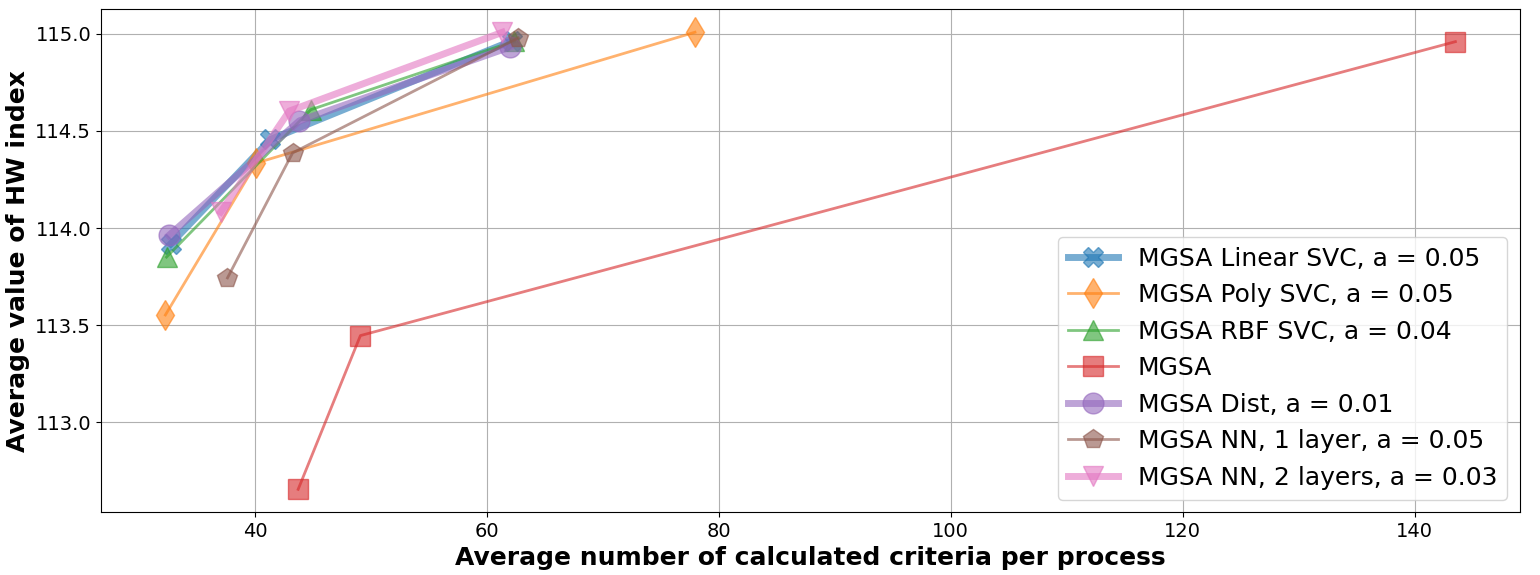
\includegraphics[width=1\linewidth]{figure/fig6.pdf} 
			\caption{Iteration speedup} %%  подпись к рисунку 
			\label{fig:fig4} 
		\end{minipage} 
	\end{center} 
\end{figure}	

\begin{table}
	\caption{Average time to solve the problem}
	\label{tab:1}
	\center
	\begin{tabular}{cccccccccccc}
		\hline\noalign{\smallskip}
		$P$ & \multicolumn{2}{c}{ $N=2$ } & & \multicolumn{2}{c}{$N=3$} & & \multicolumn{2}{c}{$N=4$} & & \multicolumn{2}{c}{$N=5$}  \\
		\noalign{\smallskip} \cline{2-3} \cline{5-6} \cline{8-9} \cline{11-12} \noalign{\smallskip}
		& \textit{Simple} & \textit{Hard} & & \textit{Simple} & \textit{Hard} & & \textit{Simple} & \textit{Hard} & & \textit{Simple} & \textit{Hard}  \\
		\noalign{\smallskip} \hline \noalign{\smallskip}
		1   & 6.35 & 12.71 & & 5.92 & 14.19 & & 31.88 & 66.29  & & 53.77 & 324.04 \\
		8   & 0.57 & 1.98  & & 1.63 & 5.59  & & 9.44  & 34.93  & & 6.62 & 52.42 \\
		16  & 1.27 & 1.71  & & 1.17 & 2.10  & & 4.71  & 8.53   & & 3.38 & 17.55 \\
		32  & 0.95 & 0.87  & & 0.38 & 0.75  & & 4.67  & 4.95   & & 1.99 & 11.48 \\
		64  & 0.21 & 1.65  & & 0.41 & 0.60  & & 5.51  & 2.93   & & 1.70 & 10.60 \\
		\noalign{\smallskip}\hline
	\end{tabular}
\end{table}

\begin{table}
	\caption{Time speedup}
	\label{tab:2}
	\center
	\begin{tabular}{cccccccccccc}
		\hline\noalign{\smallskip}
		$P$ & \multicolumn{2}{c}{ $N=2$ } & & \multicolumn{2}{c}{$N=3$} & & \multicolumn{2}{c}{$N=4$} & & \multicolumn{2}{c}{$N=5$}  \\
		\noalign{\smallskip} \cline{2-3} \cline{5-6} \cline{8-9} \cline{11-12} \noalign{\smallskip}
		& \textit{Simple} & \textit{Hard} & & \textit{Simple} & \textit{Hard} & & \textit{Simple} & \textit{Hard} & & \textit{Simple} & \textit{Hard}  \\
		\noalign{\smallskip} \hline \noalign{\smallskip}
		8  & 11.19 & 6.42  & & 3.98  & 4.01  & & 4.20 & 3.52  & & 10.80 & 10.28 \\
		16 & 5.02  & 7.43  & & 5.07  & 6.76  & & 6.77 & 7.77  & & 15.93 & 18.46 \\
		32 & 13.59 & 16.45 & & 14.97 & 22.41 & & 7.27 & 15.64 & & 31.96 & 38.76 \\
		64 & 30.42 & 7.70  & & 14.49 & 23.48 & & 5.79 & 22.61 & & 31.65 & 30.57 \\
		\noalign{\smallskip}\hline
	\end{tabular}
\end{table}


%\begin{table}[!ht]
%	\caption{Ускорениепо итерациям}
%	\label{tab:3}
%	\centering	
%	\begin{tabular}{|l|l|l|l|l|}
	%		\hline
	%		2 & 8 mpi & 16 mpi & 32 mpi & 64 mpi  \\ \hline
	%		hard & 37,61 & 49,11 & 50,04 & 34,58  \\ \hline
	%		simple & 52,06 & 19,72 & 63,02 & 307,59  \\ \hline
	%		3 & ~ & ~ & ~ &   \\ \hline
	%		hard & 15,03 & 92,04 & 47,28 & 89,74  \\ \hline
	%		simple & 10,25 & 44,70 & 44,29 & 76,87  \\ \hline
	%		4 & ~ & ~ & ~ &   \\ \hline
	%		hard & 38,14 & 106,64 & 58,40 & 117,56  \\ \hline
	%		simple & 30,75 & 79,84 & 29,41 & 40,43  \\ \hline
	%		5 & ~ & ~ & ~ &   \\ \hline
	%		hard & 162,66 & 269,09 & 201,95 & 206,94  \\ \hline
	%		simple & 46,13 & 176,70 & 98,42 & 191,00  \\ \hline
	%	\end{tabular}
%\end{table}



%Как видно из приведенных данных, присутствует ускорение по времени для задач любой размерности, при этом в целом значение ускорения не линейное, но встречается и сверхлинейное ускорение. В данных задачах большое значение имеет что, как быстро алгоритм глобального поиска поставит достаточное для дерева решения количество точек в окрестности глобального минимума, после чего локальный метод быстро находит оптимум, из за этого возникает сверхлинейное ускорение. Низкое ускорение в остальных случаях, в большей степени обусловлено тем, что алгоритм оптимизации является синхронным и на некоторых итерациях происходит ожидание завершения локального поиска, также значительным оказалось влияние накладных расходов на передачу точек между процессами. 

As can be seen from the presented data, there is a time speedup for problems of all dimensions. While the overall speedup is not linear, superlinear speedup does occur. In these problems, it is crucial how quickly the global search algorithm places enough points in the neighborhood of the global minimum for the decision tree; after this, the local method quickly finds the optimum, resulting in superlinear speedup. Lower speedup in other cases is primarily due to the synchronous nature of the optimization algorithm, leading to waiting for the completion of local searches in some iterations. The overhead of transferring points between processes also had a significant impact.


%%%%%%%%%%%%%%%%%%%%%%%%%%%%%%%%%%%%%%%%%%%%%%%%%%%%%%%%%%%%%%%%%%%%%%%%%%%%%%%%%%%%%%%%%
%%%%%%%%%%%%%%%%%%%%%%%%%%%%%%%%%%%%%%%%%%%%%%%%%%%%%%%%%%%%%%%%%%%%%%%%%%%%%%%%%%%%%%%%%
%%%%%%%%%%%%%%%%%%%%%%%%%%%%%%%%%%%%%%%%%%%%%%%%%%%%%%%%%%%%%%%%%%%%%%%%%%%%%%%%%%%%%%%%%







\section{Conclusion} 

%На данный момент в результате проделанной работы удалось совместить алгоритм глобального поиска с эффективным локальным уточнением. В отличие от известных мультистартовых схем решение о запуске локального метода принимается с помощью дерева решений. Использование такой комбинации методов позволяет значительно ускорить работу алгоритма.
%Параллельная версия алгоритма сохраняет свойства своего последовательного прототипа, что было подтверждено численными экспериментами по решению серии из нескольких сотен задач различной размерности. Предлагаемая схема позволяет использовать преимущества как распараллеливания, так и быстрого поиска локальных экстремумов.
%Помимо использования деревьев решений для выявления областей притяжения локальных экстремумов многоэкстремальных функций, мы также планируем использовать методы машинного обучения для разделения переменных решаемой задачи. Во многих прикладных задачах оптимизации зависимость целевой функции от некоторых параметров бывает либо линейной, либо одномодальной. Выделение таких переменных в специальную группу и решение задачи с помощью параллельной схемы рекурсивной оптимизации \cite{Barkalov2020_1} позволяет сократить время решения задачи на порядки по сравнению с использованием глобального поиска сразу по всем переменным.

Currently, the work done has made it possible to combine a global search algorithm with effective local refinement. Unlike known multi-start schemes, the decision to launch the local method is made using a decision tree. The use of such a combination of methods significantly speeds up the algorithm.

The parallel version of the algorithm retains the properties of its sequential prototype, which was confirmed by numerical experiments on solving a series of several hundred problems of various dimensions. The proposed scheme allows us to exploit the advantages of both parallelization and rapid local extrema search.

In addition to using decision trees to identify the basins of attraction of local extrema of multimodal functions, we also plan to use machine learning methods to separate the variables of the problem being solved. In many applied optimization problems, the dependence of the objective function on some parameters is either linear or unimodal. Identifying such variables into a special group and solving the problem using a parallel recursive optimization scheme \cite{Barkalov2020_1} can reduce the solution time by orders of magnitude compared to using global search across all variables at once.

%%%%%%%%%%%%%%%%%%%%%%%%%%%%%%%%%%%%%%%%%%%%%%%%%%%%%%%%%%%%%%%%%%%%%%%%%%%%%%%%%%%%%%%%%
%%%%%%%%%%%%%%%%%%%%%%%%%%%%%%%%%%%%%%%%%%%%%%%%%%%%%%%%%%%%%%%%%%%%%%%%%%%%%%%%%%%%%%%%%
%%%%%%%%%%%%%%%%%%%%%%%%%%%%%%%%%%%%%%%%%%%%%%%%%%%%%%%%%%%%%%%%%%%%%%%%%%%%%%%%%%%%%%%%%


\begin{credits}
	\subsubsection{\ackname} This study was supported by the Ministry of Science and Higher Education of the Russian Federation, project no. FSWR-2023-0034.
	
	\subsubsection{\discintname}
	The authors have no competing interests to declare that are	relevant to the content of this article.
\end{credits}

%%%%%%%%%%%%%%%%%%%%%%%%%%%%%%%%%%%%%%%%%%%%%%%%%%%%%%%%%%%%%%%%%%%%%%%%%%%%%%%%%%%%%%%%%
%%%%%%%%%%%%%%%%%%%%%%%%%%%%%%%%%%%%%%%%%%%%%%%%%%%%%%%%%%%%%%%%%%%%%%%%%%%%%%%%%%%%%%%%%
%%%%%%%%%%%%%%%%%%%%%%%%%%%%%%%%%%%%%%%%%%%%%%%%%%%%%%%%%%%%%%%%%%%%%%%%%%%%%%%%%%%%%%%%%


%
% ---- Bibliography ----
%
\bibliographystyle{spmpsci}
\bibliography{bibliography}{}











\end{document}
